\documentclass[12pt]{article}
\usepackage[inner=2.0cm,outer=2.0cm,top=2.5cm,bottom=2.5cm]{geometry}
\usepackage{float}
\usepackage{graphicx}
\usepackage{hyperref}
\setlength\voffset{-0.25in}
\setlength\textheight{675pt}

\usepackage{titling}
\setlength{\droptitle}{19em}
\title{CS 3651 - Prototyping Intelligent Devices\\ Project Documentation\\Wall-E}
\author{Names: Tri Le, Nithya Jayakumar}
\date{\today}


\begin{document}
\maketitle

\newpage
\begin{itemize}
    \item[1)] \textbf{Baby Wall-E}
    \begin{itemize}
        \item[a)] Wall-E Hardware:
        \begin{itemize}
            \item[1)] Arduino Nano [x1]: This is the primary microcontroller; the Arduino Nano will execute the robot’s code, coordinating various actions and responses.
            \item[2)] Buck Converter [x2]: Voltage converter from the 4 AA batteries to the Arduino, motors, LEDs, and other electronic parts; and from the 9V battery to the servos.
            \item[3)] DC Gear Motors 3-6V, 52RPM - 104RPM [x2]: These motors will drive the wheels, allowing the robot to move forward, backward, and turn in response to objects detected by the ultrasonic sensor and the infrared sensors installed at the robot's eye.
            \item[4)] Servos [x3]: These will control the movement of the robot’s head rotation and arms. Servos add dynamic and expressive qualities to the robot’s appearance.
            \item[5)] Ultrasonic Sensor [x1]: This sensor allows the robot to detect obstacles and avoid them, enabling safe movement.
            \item[6)] Infrared Sensors (IR) [x2]: These sensors are placed at the robot's eye. They allow the user to interact with the robot, for example, by making hand movements in front of the robot, which enables the robot to rotate its head and body towards the hand.
            \begin{figure}[H]
                \centering
                \includegraphics[width=550pt]{Wall-EParts.png}
                \caption{Baby Wall-E Hardware Details}
                \label{fig:enter-label}
            \end{figure}
            \item[7)] Buzzer [x1]: This will produce sounds for the robot.
            \item[8)] H-Bridge [x1]: This is responsible for controlling the DC motors that drive the robot’s movement. The H-Bridge facilitates precise control over speed and direction.
            \item[9)] Red, Yellow, and Green LEDs [x1]: These LEDs will serve as a battery level indicator. Since Wall-E has a battery level display, this somewhat serves the same purpose.
            \item[10)] Blue and White LEDs [x2 for each eye]: These LEDs will represent the robot's eyes. Normally they are blue, but they will change to white when an object is detected.
            \item[11)] Red LED [x1]: To indicate that there is power from the 9V battery to the servos.
        \end{itemize}
        
        \item[b)] Libraries that use in code:\\
            We coded everything ourselves. The only two libraries we used for the code are: Servo.h and NewPing.h
            \begin{figure}[H]
                \centering
                \includegraphics[width=200pt]{code_library.png}\
                \label{fig:enter-label}
            \end{figure}
            \begin{itemize}
                \item[+] \textbf{Servo.h} played a crucial role in controlling the movement of the servos responsible for the arms and head of the robot. With Servo.h, we were able to precisely adjust the position and movement of these components, allowing for dynamic and expressive gestures that enhanced the overall interaction and appeal of baby Wall-E.
                \item[+] \textbf{NewPing.h} managing the ultrasonic sensor, a important component for obstacle detection and navigation. And by using the NewPing.h, we were able to effectively interface with the ultrasonic sensor, enabling our robot to detect obstacles in its environment and navigate safely.
            \end{itemize}
        
        \item[c)] Parts that the team modify:
        \begin{itemize}
            \item[+] The team didn't design the Wall-E CAD files ourselves. Fortunately, we found existing designs for Baby Wall-E (\href{https://www.thingiverse.com/thing:5957438}{link}). Due to the complexity of the CAD files, we were unable to make extensive modifications, but instead, we resized the robot to be larger than the original.
            \\ - After printing, we modified it by drilling holes to accommodate the ultrasonic sensor, as well as adjusting the eyes to incorporate LED lights and infrared sensors.
            \begin{figure}[H]
                \centering
                \includegraphics[width=350pt]{Modify_parts.png}
                \caption{Modified Components for Baby Wall-E}
                \label{fig:enter-label}
            \end{figure}
            \item[+] Some components that the team created ourselves include power switches for the batteries, a buzzer for generating sound, LED lights for the eyes, a LED battery indicator, and sensors. As mentioned before, we coded the entire project ourselves, without relying on external resources.
        \end{itemize}
        
        \item[d)] Skills learned to accomplish the project:
            \begin{itemize}
                \item[+] To be able to complete this project, the team learned how to:
                \begin{enumerate}
                    \item Use a buck converter to obtain the correct voltage for the Arduino and other components.
                    \item Document all electronic components, such as creating an electronic schematic showing how the parts are connected to each other, including the labels of pins on the Arduino. This allows the team to navigate through multiple phases, such as during setup and soldering, ensuring that all wires are connected correctly.
                    \item Decide and plan where all hardware parts will be wired and soldered.
                    \item Understand what is wrong with the project, such as when the robot appears to not be working correctly. It took more than one week to understand what happened. It turned out that the battery was low, causing the robot to not move as expected.
                \end{enumerate}
            \end{itemize}

        
        \item[e)] The process to make Baby Wall-E:
        \begin{itemize}
            \item[1)] Initial testing performed:
            \begin{enumerate}
                \item[a)] Initially, we tested everything on a protoboard, including the ultrasonic sensor, servos, and motors. Then, we coded everything and ensured that everything worked.
                \begin{figure}[H]
                    \centering
                    \includegraphics[width=100pt]{phase0.png}
                    \caption{Baby Wall-E Initial Hardware Testing Phase}
                    \label{fig:phase0}
                \end{figure}
                \item[b)] Next, we worked on the LEDs for the eyes to easily indicate when an obstacle is detected. We then placed everything into a box to test the code and the movements of all components.
                \begin{figure}[H]
                    \centering
                    \includegraphics[width=110pt]{phase1.png}
                    \caption{Testing Baby Wall-E's Code and Movement Functions}
                    \label{fig:phase1}
                \end{figure}
            
                \item[c)] After confirming that everything ran smoothly, we then worked on the 3D printing parts. Once the parts were available, we assembled everything, including soldering all the hardware. We also added more hardware such as IR sensors and a battery indicator, and coded them to ensure they were also working.
                \begin{figure}[H]
                    \centering
                    \begin{minipage}[t]{0.45\textwidth}
                        \centering
                        \includegraphics[width=100pt]{phase2.png}
                        \caption{Testing Baby Wall-E's Movement on 3D Printed Body}
                        \label{fig:phase2}
                    \end{minipage}\hfill
                    \begin{minipage}[t]{0.45\textwidth}
                        \centering
                        \includegraphics[width=100pt]{phase3.png}
                        \caption{Infrared Sensor Testing for Baby Wall-E}
                        \label{fig:phase3}
                    \end{minipage}
                \end{figure}
            \end{enumerate}

            \begin{figure}[H]
                \centering
                \includegraphics[width=100pt]{phase3.2.png}
                \caption{Setting Up Baby Wall-E's 3D Printed Tracks}
                \label{fig:phase3.2}
            \end{figure}
            
            \item[2)] Ideas that didn't pan out
            \begin{enumerate}
                \item[a)] As mentioned in the project proposal, the team expressed interest in implementing voice control. However, this plan did not materialize as expected. The team encountered motor problems, which resulted in a pause in the robot's development for almost a week.
                
                \item[b)] The issue with the wheels stemmed from the printed tracks for the robot not functioning properly because the motor axles were not long enough to hold them. The team made various attempts to remedy this, including using hot glue and epoxy (as recommended by the PI in the Mechanical Makerspace). However, these approaches proved ineffective.
                \begin{figure}[H]
                    \centering
                    \begin{minipage}[t]{0.45\textwidth}
                        \centering
                        \includegraphics[width=100pt]{trackfix0.png}
                        \caption{Track Issue Resolved with Metal Reinforcement}
                        \label{fig:trackfix0}
                    \end{minipage}\hfill
                    \begin{minipage}[t]{0.45\textwidth}
                        \centering
                        \includegraphics[width=100pt]{trackfix1.png}
                        \caption{The Piece of Metal Perfectly Fits the Motor Axle}
                        \label{fig:trackfix1}
                    \end{minipage}
                \end{figure}
                Subsequently, the team tried using a piece of metal that perfectly fit the motor axle and was sturdy enough to hold the tracks. Unfortunately, the motors were not powerful enough to move the tracks, and as a result, one of the motors overheated and broke free from the hot glue that secured it inside the robot. Ultimately, we decided to switch to using robot wheels instead.
                \begin{figure}[H]
                    \centering
                    \begin{minipage}[t]{0.45\textwidth}
                        \centering
                        \includegraphics[width=100pt]{wheels.png}
                        \caption{The Track Experienced Fitting Issues and Snapped Midway}
                        \label{fig:trackfix0}
                    \end{minipage}\hfill
                    \begin{minipage}[t]{0.45\textwidth}
                        \centering
                        \includegraphics[width=100pt]{track_printed.png}
                        \caption{The Printed Track Experienced Fitting Issues}
                        \label{fig:trackfix1}
                    \end{minipage}
                \end{figure}
            \end{enumerate}
            
            \item[3)] Hardware that had to be changed
            \begin{enumerate}
                \item[+] The only hardware we had to change was the battery. Initially, we had only one 4 AA battery powering everything, including the Arduino, servos, and other components.
                However, as the team observed, this caused numerous problems and led to confusion. Despite the Arduino functioning properly when connected to a computer, using the battery— even a new one— resulted in erratic behavior by the robot. For instance, it would turn on and then immediately turn off. It took the team almost a week to figure out the cause, especially after adding additional IR sensors towards the end of the project. Consequently, we decided to use two separate batteries: one to power the Arduino and other components, and another for the servos.
                \begin{figure}[H]
                    \centering
                    \includegraphics[width=130pt]{battery.png}
                    \caption{Baby Wall-E Battery Storage for Easy Replacement}
                    \label{fig:battery}
                \end{figure}
            \end{enumerate}
            
            \item[4)] Lessons learned
            \begin{enumerate}
                \item[+] One important lesson the team learned is not to oversolder, as this can cause wires to melt and break without notice. During our soldering process, some wires were accidentally broken and not initially visible. Consequently, we had to resolder, during which we discovered that two wires for the H-bridge were burned and not connected to the Arduino.
                \item[+] Additionally, we learned that connectors like the ones used for the motors are not strong enough. With a strong pull, it is possible to pull the wire out from the motor. This happened to us after we had assembled everything. We had to disassemble everything and hot glue a new motor in place. From this experience, we learned to add extra solder to those pre-soldered purchased parts and apply hot glue over them, as it may hold the wire better.
            \end{enumerate}

        \end{itemize}
        \item[f)] Baby Wall-E, fully assembled:
        \begin{figure}[H]
            \centering
            \includegraphics[width=130pt]{wall_e.png}
            \caption{Baby Wall-E}
            \label{fig:battery}
        \end{figure}
        
    \end{itemize}
    \item[2)] \textbf{Demo Videos}
    \begin{itemize}
        \item[1)] Wall-E Initial Setup - \href{https://youtube.com/shorts/i2jB2JJ8H8I?feature=share}{https://youtube.com/shorts/i2jB2JJ8H8I?feature=share}
        \\- This video demonstrates the purpose of the initial testing phase on the code, showing how the device moves when an obstacle is detected. The hardware is placed inside an empty iPhone box, with wheels attached to observe the movement.
        
        \item[2)] Wall-E Obstacle Detect - \href{https://youtube.com/shorts/-GJ3NuQVtVU?feature=share}{https://youtube.com/shorts/-GJ3NuQVtVU?feature=share}
        \\- This video demonstrates how the Baby Wall-E detects obstacles using an ultrasonic sensor. Initially, the robot detects the toolbox, and when an obstacle is detected, the white LED lights up to indicate its presence. It continues to turn until no obstacles are detected. Additionally, the robot emits noise when an obstacle is detected. Moreover, the video highlights how the Baby Wall-E moves its head and arms.
        
        \item[3)] Wall-E Detects Walls - \href{https://youtube.com/shorts/RRByPIQfrT4?feature=share}{https://youtube.com/shorts/RRByPIQfrT4?feature=share}
        \\- This video illustrates how IR sensors and ultrasonic sensors work together. At the beginning, after the ultrasonic sensor detects a wall, the device turns around. It continues to rotate until it finds sufficient distance to move freely.
        
        \item[4)] Wall-E Dectect Hand - \href{https://youtube.com/shorts/QcuA5vfDQpo?feature=share}{https://youtube.com/shorts/QcuA5vfDQpo?feature=share}
        \\- This video demonstrates how the Baby Wall-E utilizes its infrared sensors, placed in its eyes, to detect nearby movement in front of them. This showcases the interactive aspect of how users can interact with Wall-E. As shown, when you place your hand near Wall-E's eye, it stops moving forward and turns its head toward the hand, moving its body in that direction.
    \end{itemize}

    \item[3)] \textbf{Schematics/Electrical Block Diagrams}
    \begin{itemize}
        \item Before fixing the issues with the battery
            \begin{figure}[H]
                \centering
                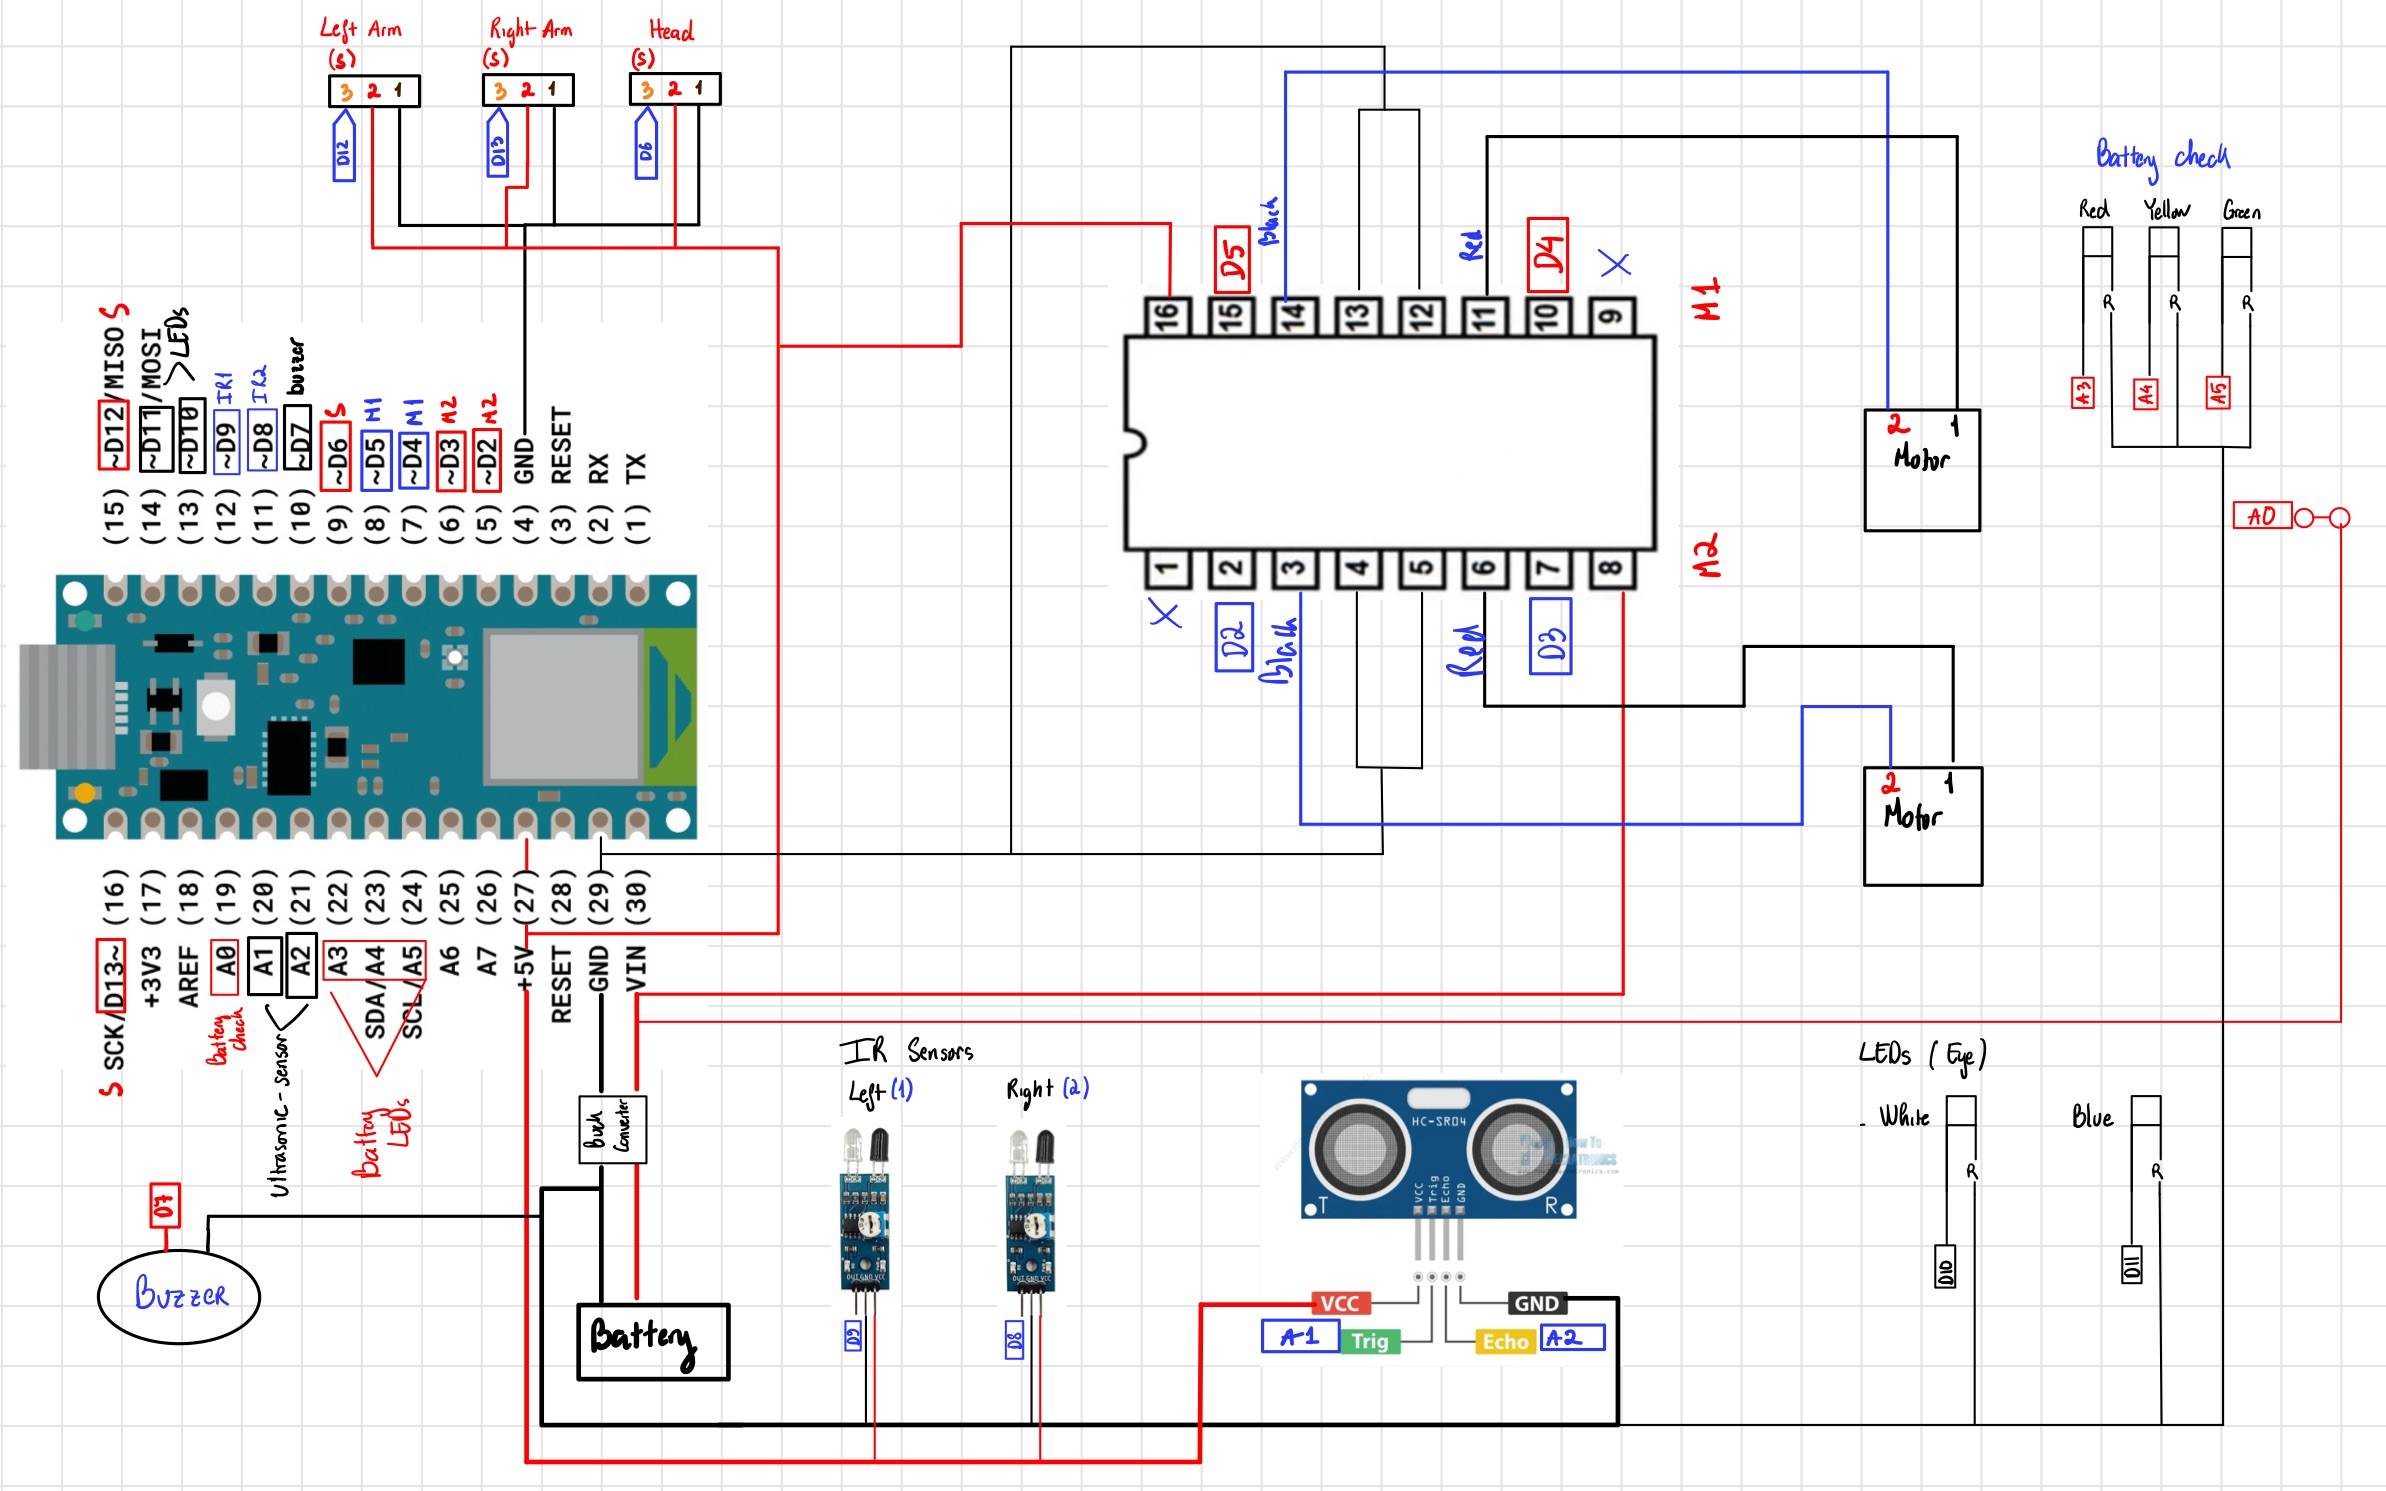
\includegraphics[width=300pt]{Project-1.jpg}
                \caption{Baby Wall-E Hardware/Electronic Schematic Prior to Adding Second Battery}
                \label{fig:schematic1}
            \end{figure}
        \item After understanding the issue and adding an additional battery
            \begin{figure}[H]
                \centering
                \includegraphics[width=300pt]{Project-3.jpg}
                \caption{Baby Wall-E Hardware/Electronic Schematic After Addition of Second Battery}
                \label{fig:schematic2}
            \end{figure}
    \end{itemize}

    \item[4)] \textbf{Resources Used}
    \begin{enumerate}
        \item[+] The primary resource we utilized for this project was a series of YouTube videos. While we didn't follow the exact instructions, these videos provided valuable guidance and inspiration, especially in the initial stages of our project. Instead of utilizing Bluetooth for robot control, as demonstrated in the videos, we opted to incorporate ultrasonic and infrared sensors for obstacle detection and avoidance.
        \begin{itemize}
            \item DIY fully functional mini Wall-E using Arduino Nano - \href{https://www.youtube.com/watch?v=iaqVNqsvQwI}{link} \& \href{https://www.youtube.com/watch?v=Cqv2w0qYf-s}{link}
            \& \href{https://www.thingiverse.com/thing:5957438/files}{STL files}
        \end{itemize}
        
        The main aspect we borrowed from these resources was the 3D files for the outer structure of Wall-E. Since our team had limited experience in CAD design, these files proved invaluable in quickly adapting and modifying the design to accommodate other components such as sensors and LEDs.
    \end{enumerate}
        
    \item[5)] \textbf{Group Work}
    \begin{enumerate}
        \item[+] We collaborated closely on this project, meeting 3 to 4 times per week to progress our work. Additionally, we dedicated two weeks at the Hive, meeting daily to focus on assembling the robot and working on the 3D printed parts.
        \item[+] Our typical approach involved working on the physical robot together during our meetings. In between meetings, we would individually focus on coding tasks, utilizing GitHub for code sharing and updates to keep each other informed of our progress.
    \end{enumerate}

    \item \textbf{Conclusion}: The team successfully recreated the beloved character Wall-E, surpassing our initial goals by assembling all 3D printed parts to resemble the iconic robot. While the final result may not match our exact expectations, such as the tracks which could have been improved with better motors, we encountered challenges that led to valuable learning experiences. For instance, when the tracks did not fit and broke midway, we attempted various solutions, including seeking assistance from the Mechanical Makerspace and using epoxy E6000, although this did not yield the desired outcome. This setback prompted us to pause our work for a week. However, we adapted by utilizing normal wheels as a backup plan. Given more time, we could have redesigned the electronic and hardware schematic and opted for better batteries and motors. Despite these challenges, we believe our project was successful. We appreciate the opportunity to work on this project and thank you for a great semester!
\end{itemize}
\end{document}